\chapter{Unified Model}

\section{Families of Markov Chains}
This thesis considers a~parametric transition probability function as an~explicit representation of an~MCs family.
Such explicit representation relieves the~presentation and provides to describe exciting and practical problems for probabilistic synthesis.
On the~other hand,~arbitrary probabilistic programs permit the~modelling of more complex and independent parameter structures~\cite{cegar}.
In this thesis and our implementation,~we consider a~more flexible high-level modelling language,~see Section~\todo{?}.

\begin{definition}[Family of MCs]
\cite{cegar}
    A~\emph{family of MCs} $\fml$ is a~quadruple $\family$  where $S$ is a~finite set of \emph{states}, $\sinit \in S$ is an~\emph{initial state},~$K$ is a~finite set of parameters with domains $T_k \subseteq S$ for each $k \in K$,~and $\fpm : S \rightarrow Distr(K)$ is a~family of transition probability functions.
\end{definition}

The~transition probability function $\fpm$ of MCs family $\fml$ maps each state $s \in S$ to the~probability distribution over parameters from $K$.
As we mentioned above,~these parameters represent undefined system specifications when the~probabilistic synthesis is considered.
This function $\fpm$ yields a~specific MC when we instantiate each parameter $k \in K$ with the~specific value from its domain $T_k \subseteq S$.
We call such instantiated MC as \textit{realisation},~and the~following definition describes it.

\begin{definition}[Realisation]
\cite{cegar}
A~\emph{realization} of a~family $\fml = \family$ of MCs is a~function $r: K \rightarrow S$ s.t.~$\forall k \in K :  r(k) \in T_k$. 
A~realization~$r$ yields a MC $\fmlr = (S,\sinit,\fpm(r))$,~where $\fpm(r)$ represents the~transition probability matrix where each parameter $k \in K$ is substituted with $r(k)$. 
Let $\rlzf$ denote the~set of all realisations for $\fml$.
\end{definition}

A~set $\prod_{k \in K} T_k$ representing all possible parameter combinations values has the~same semantics as a~set $\rlzf$ representing all family realisations.
In other words,~we can define the~\textit{size of the family} of MCs in the~following way: $\lvert \fml \rvert := \lvert \prod_{k \in K} T_k \rvert = \lvert \rlzf \rvert = \prod_{k \in K} \lvert T_k \rvert$.
The~family size $\lvert \fml \rvert$ is finite because of the~finiteness of each parameter domain $T_k \subseteq S$,~but it is exponential in the~number of parameters $\lvert K \rvert$.
We note $\rlz$ as the~sub-families induced from the~whole family $\rlzf$.
The~individual MCs within the~family share the~same state space $S$,~but their set of reachable states can vary.

\begin{example}[Family of MCs]\label{exam:mcfamily}
Let $\fml = \family$ be a~family of MCs,~where $S = \{s_0, s_1, s_2, s_3\}$ and $K = \{ k_0, k_1\}$ with domains $T_{k_0} = \{s_0, s_2\}$,~and $T_{k_1} = \{s_1, s_3\}$.
The parametric transition function $\fpm$ is defined as follows:
\begin{align*}
    \fpm(s_0) &= 0.5 : k_0 + 0.5 : k_1  &  \fpm(s_1)  &= 0.5 : k_1  + 0.5 : k_0 \\
    \fpm(s_2) &= 1.0: k_1   &  \fpm(s_3)  &= 1.0 : s_3
\end{align*}
Figure~\ref{fig:mcfamily} draws the~MCs family $\fml$ that correspond to all possible realisations: $\lvert T_{k_0} \rvert \cdot \lvert T_{k_1} \rvert = 2 \cdot 2 = 4$.
We note that these MCs have a~different topology of the~underlying state space,~resulting in different sets of reachable states.
\end{example}

\begin{figure}[ht!]
\centering
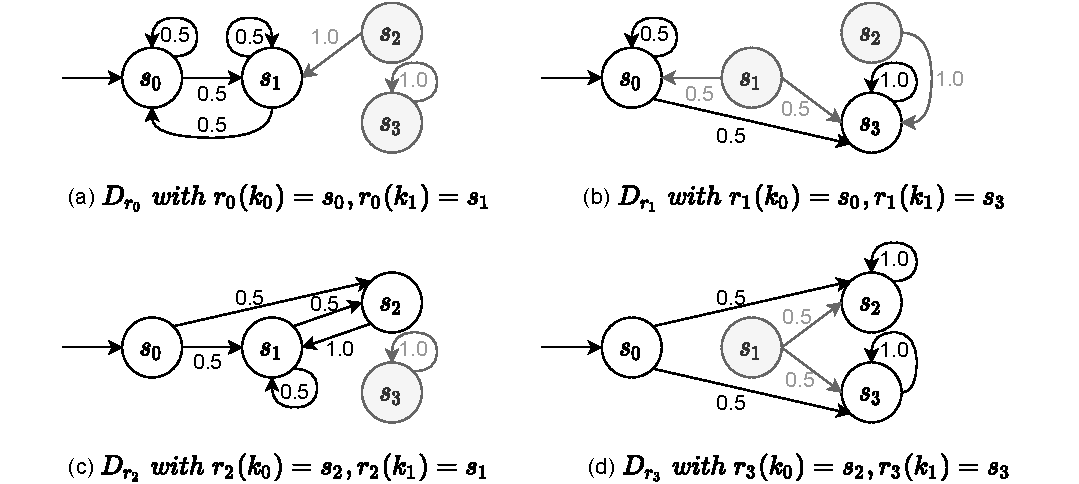
\includegraphics[width=0.9\textwidth]{figures/MCFamily.pdf}
\caption{A family $\fml$ of four various realisations. Unreachable states are greyed out.}%
\label{fig:mcfamily}%
\end{figure}

\textit{Quotient} MDP $M^\fml$ simulates the~behaviours of each member of the~family $\fml$ and can even pass between them during the~execution.
In more precise,~when the~path $s_0s_1s_2 \dots$ is executable in some family member $D_r$,~then it is also executable in $M^\fml$ as $s_0 \overset{r}{\rightarrow} s_1 \overset{r}{\rightarrow} \dots$.
However,~there may exist a~path $\pi$ that is executable in $M^\fml$,~but it is not realisable in neither of the~family members.
We can conclude that \textit{quotient} MDP over-approximates the~behaviours of the~members of family $\fml$.

\begin{definition}[Quotient MDP] \label{def:quotient_mdp}
\cite{roman-DP}
Let $\fml = \family$ be an~MCs family.
A~\textit{quotient} MDP $M^\fml$ of the~family $\fml$ is a~tuple $(S, s_{init}, \mathcal{R}^\fml, \mathcal{P})$,~where $\mathcal{P}(\cdot)(r) \equiv \mathcal{B}_r$.
\end{definition}

A~restriction of a~\textit{quotient} MDP concerning $\rlz \subseteq \rlz^\fml$ induces an~MDP which takes into account only transitions associated with $\rlz$.
We define the~usage of \textit{consistent} schedulers ensuring that execution of a~\textit{quotient} MDP always selects the~concrete realisation.
We note that a~\textit{consistent} scheduler yields a~specific family member for a~\textit{quotient} MDP,~which directly follows from Definition~\ref{def:quotient_mdp}.

\begin{definition}[Consistent scheduler]
\cite{roman-DP}
Let $\fml = \family$ be a~MCs family and let $M^\fml = (S, s_{init}, \mathcal{R}^\fml, \mathcal{P})$ be a quotient MDP of the~family $\fml$.
For $r \in \rlz^\fml$,~a (memory-less) scheduler $\sigma_r \in \sigma^{M^\fml}$ is called \textit{r-consistent} iff $\forall s \in S: \, \sigma(s) = r$.
A~scheduler is called \textit{consistent} iff it is consistent for some $r \in \rlz^\fml$.
\end{definition}